\fenicschapter{The finite element method}
              {The finite element method}
              {The finite element method}
              {Robert C. Kirby and Anders Logg}
              {kirby-7}

The finite element method has emerged as a universal method for the
solution of differential equations. Much of the success of the finite
element method can be attributed to its generality and elegance,
allowing a wide range of differential equations from all areas of
science to be analyzed and solved within a common framework. Another
contributing factor to the success of the finite element method is the
flexibility of formulation, allowing the properties of the
discretization to be controlled by the choice of approximating finite
element spaces.

In this chapter, we review the finite element method and summarize
some basic concepts and notation used throughout this book. In the
coming chapters, we discuss these concepts in more detail, with a
particular focus on the implementation and automation of the finite
element method as part of the FEniCS Project.

%------------------------------------------------------------------------------
\section{A simple model problem}
\index{Poisson's equation}
\index{boundary conditions}

In 1813, Sim\'eon Denis Poisson published in \emph{Bulletin de la
soci\'et\'e philomatique} his famous equation as a correction of
an equation published earlier by Pierre-Simon Laplace. Poisson's
equation is a second-order partial differential equation stating that
the negative Laplacian $-\Delta u$ of some unknown field $u = u(x)$ is
equal to a given function $f = f(x)$ on a domain~$\Omega \subset \R^d$,
possibly amended by a set of boundary conditions for the solution $u$
on the boundary $\partial \Omega$ of~$\Omega$:
\index{Dirichlet condition}
\index{Neumann condition}
\begin{equation} \label{eq:poisson}
  \begin{split}
    - \Delta u &= f \,\,\, \quad \mbox{in } \Omega,
    \\
    u &= u_0 \quad \mbox{on } \Gamma_{\mathrm{D}} \subset \partial \Omega,
    \\
    - \partial_n u &= g \,\,\, \quad \mbox{on } \Gamma_{\mathrm{N}} \subset \partial \Omega.
  \end{split}
\end{equation}
The Dirichlet boundary condition $u = u_0$ signifies a prescribed
value for the unknown~$u$ on a subset $\Gamma_{\mathrm{D}}$ of the
boundary, and the Neumann boundary condition $-\partial_n u = g$
signifies a prescribed value for the (negative) normal derivative of
$u$ on the remaining boundary $\Gamma_{\mathrm{N}} = \partial \Omega
\setminus \Gamma_{\mathrm{D}}$. Poisson's equation is a simple model
for gravity, electromagnetism, heat transfer, fluid flow, and many
other physical processes. It also appears as the basic building block
in a large number of more complex physical models, including the
Navier--Stokes equations which we return to in
Chapters~\ref{chap:terrel}, \ref{chap:kvs-1},
\ref{chap:mortensen},
\ref{chap:kvs-2}, \ref{chap:hentschel}, \ref{chap:lopes},
 \ref{chap:hoffman-1} and \ref{chap:selim}.

To derive Poisson's equation~(\ref{eq:poisson}), we may consider a
model for the temperature $u$ in a body occupying a domain~$\Omega$
subject to a heat source $f$. Letting $\sigma = \sigma(x)$ denote heat
flux, it follows by conservation of energy that the outflow of energy
over the boundary $\partial\omega$ of any test volume
$\omega\subset\Omega$ must be balanced by the energy emitted by the
heat source $f$:
\begin{equation}
  \int_{\partial\omega} \sigma \cdot n \ds = \int_{\omega} f \dx.
\end{equation}
Integrating by parts, we find that
\begin{equation} \label{eq:testvolume}
  \int_{\omega} \nabla \cdot \sigma \dx = \int_{\omega} f \dx.
\end{equation}
Since~\eqref{eq:testvolume} holds for all test volumes
$\omega \subset \Omega$, it follows that $\nabla \cdot \sigma = f$
throughout $\Omega$ (with suitable regularity assumptions on $\sigma$
and $f$). If we now make the assumption that the heat flux~$\sigma$ is
proportional to the negative gradient of the temperature $u$
(Fourier's law), \index{Fourier's law}
\begin{equation}
  \sigma = -\kappa \nabla u,
\end{equation}
we arrive at
the following system of equations:
\begin{equation}
\label{eq:poisson,mixed}
  \begin{split}
    \nabla \cdot \sigma &= f \quad \mbox{in } \Omega, \\
    \sigma + \nabla u   &= 0   \quad \mbox{in } \Omega,
\end{split}
\end{equation}
where we have assumed that the heat conductivity is $\kappa = 1$.
Replacing $\sigma$ in the first of these equations by $-\nabla u$, we
arrive at Poisson's equation~(\ref{eq:poisson}). Note that one may as
well arrive at the system of first-order
equations~(\ref{eq:poisson,mixed}) by introducing~$\sigma = -\nabla u$
as an auxiliary variable in the second-order
equation~(\ref{eq:poisson}). We also note that the Dirichlet and
Neumann boundary conditions in~(\ref{eq:poisson}) correspond to
prescribed values for the temperature and heat flux, respectively.

\begin{figure}
\bwfig
%  \centering
%  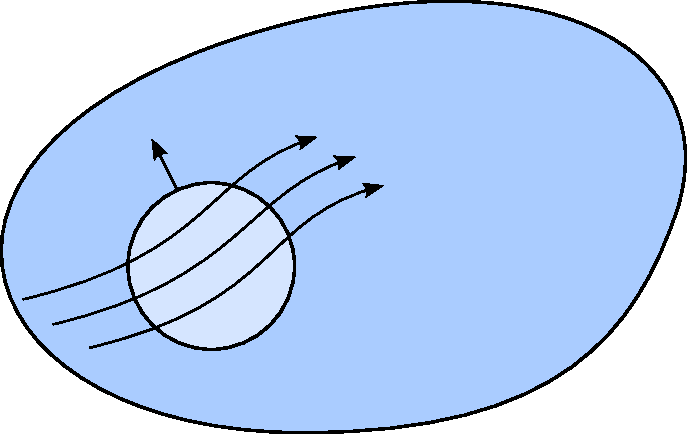
\includegraphics[width=\smallfig]{chapters/kirby-7/pdf/heat_equation_model_domain.tex}
  \fenicsfig{kirby-7}{heat_equation_model_domain}{\smallfig}
  \caption{Poisson's equation is a simple consequence of balance of
    energy in an arbitrary test volume~$\omega \subset \Omega$.}
\end{figure}

%------------------------------------------------------------------------------
\section{Finite element discretization}
\index{finite element discretization}

\subsection{Discretizing Poisson's equation}

To discretize Poisson's equation~(\ref{eq:poisson}) by the finite
element method, we first multiply by a test function $v$ and integrate
by parts to obtain
\begin{equation}
  \int_{\Omega} \nabla u \cdot \nabla v \dx
  - \int_{\partial \Omega} \partial_n u \, v \ds
  =
  \int_{\Omega} f v \dx.
\end{equation}
Letting the test function~$v$ vanish on the Dirichlet boundary
$\Gamma_{\mathrm{D}}$ where the solution $u$ is known, we arrive at
the following classical variational problem: find $u \in V$ such that
\begin{equation} \label{eq:poisson,varproblem}
  \int_{\Omega} \nabla u \cdot \nabla v \dx =
  \int_{\Omega} f v \dx - \int_{\Gamma_{\mathrm{N}}} g v \ds
  \quad \foralls v \in \hat{V}.
\end{equation}
The test space $\hat{V}$ is defined by
\begin{equation}
  \hat{V} = \{v \in H^1(\Omega) : v = 0 \mbox{ on } \Gamma_{\mathrm{D}}\},
\end{equation}
and the trial space \( V \) contains members of \( \hat{V} \) shifted
by the Dirichlet condition:
\begin{equation}
  V = \{ v \in H^1(\Omega) : v = u_0 \mbox{ on } \Gamma_{\mathrm{D}} \}.
\end{equation}

We may now discretize Poisson's equation by restricting the
variational problem~(\ref{eq:poisson,varproblem}) to a pair of
discrete spaces: find $u_h \in V_h \subset V$ such that
\begin{equation} \label{eq:poisson,varproblem,discrete}
  \int_{\Omega} \nabla u_h \cdot \nabla v \dx =
  \int_{\Omega} f v \dx - \int_{\Gamma_{\mathrm{N}}} g v \ds
  \quad \foralls v \in \hat{V}_h \subset \hat{V}.
\end{equation}
We note here that the Dirichlet condition $u = u_0$ on
$\Gamma_{\mathrm{D}}$ enters directly into the definition of the trial
space~$V_h$ (it is an \emph{essential} boundary condition), whereas
the Neumann condition $-\partial_n u = g$ on $\Gamma_{\mathrm{N}}$
enters into the variational problem (it is a \emph{natural} boundary
condition).

To solve the discrete variational
problem~(\ref{eq:poisson,varproblem,discrete}), we must construct a
suitable pair of discrete trial and test spaces $V_h$ and $\hat{V}_h$.
We return to this issue below, but assume for now that we have a basis
$\{\phi_j\}_{j=1}^N$ for $V_h$ and a basis $\{\hat{\phi}_i\}_{i=1}^N$
for $\hat{V}_h$. Here, $N$ denotes the dimension of the spaces~$V_h$ and $\hat{V}_h$.
We may then make an Ansatz for $u_h$ in terms of the basis functions
of the trial space,
%
\index{finite element solution}
\index{finite element space}
%
\begin{equation}
  u_h(x) = \sum_{j=1}^N U_j \phi_j(x),
\end{equation}
where $U \in \R^N$ is the vector of degrees of freedom to be computed.
Inserting this into~(\ref{eq:poisson,varproblem,discrete}) and varying
the test function $v$ over the basis functions of the discrete test
space $\hat{V}_h$, we obtain
\begin{equation}
  \sum_{j=1}^N U_j \int_{\Omega} \nabla \phi_j \cdot \nabla \hat{\phi}_i \dx =
  \int_{\Omega} f \hat{\phi}_i \dx - \int_{\Gamma_{\mathrm{N}}} g \hat{\phi}_i \ds,
  \quad i = 1,2,\ldots,N.
\end{equation}
We may thus compute the finite element solution $u_h = \sum_{j=1}^N
U_j \phi_j$ by solving the linear system
\begin{equation}
  AU = b,
\end{equation}
where
\begin{equation}
\begin{split}
  A_{ij} &= \int_{\Omega} \nabla \phi_j \cdot \nabla \hat{\phi}_i \dx,
  \\
  b_i &= \int_{\Omega} f \hat{\phi}_i \dx - \int_{\Gamma_{\mathrm{N}}} g \hat{\phi}_i \ds.
\end{split}
\end{equation}

\subsection{Discretizing the first-order system}
\label{sec:kirby-7:mixed}
\index{mixed problem}

We may similarly discretize the first-order
system~(\ref{eq:poisson,mixed}) by multiplying the first equation by a
test function $v$ and the second equation by a test function
$\tau$. Summing up and integrating by parts, we find that
\begin{equation}
  \int_{\Omega} (\nabla \cdot \sigma) \, v + \sigma \cdot \tau
  - u \nabla \cdot \tau \dx +
  \int_{\partial\Omega} u \tau \cdot n \ds
  = \int_{\Omega} f v \dx
  \quad \foralls (v, \tau) \in \hat{V}.
\end{equation}
The normal flux $\sigma \cdot n = g$ is known on the Neumann
boundary~$\Gamma_{\mathrm{N}}$ so we may take $\tau \cdot n = 0$
on~$\Gamma_{\mathrm{N}}$.  Inserting the value for $u$ on the
Dirichlet boundary~$\Gamma_{\mathrm{D}}$, we arrive at the following
variational problem: find $(u, \sigma) \in V$ such that
\begin{equation} \label{eq:poisson,varproblem,mixed}
  \int_{\Omega} (\nabla \cdot \sigma) \, v + \sigma \cdot \tau
  - u \nabla \cdot \tau \dx
  = \int_{\Omega} f v \dx - \int_{\Gamma_{\mathrm{D}}} u_0 \tau \cdot n \ds
  \quad \foralls (v, \tau) \in \hat{V}.
\end{equation}
A suitable choice of trial and test spaces is
\begin{equation}
  \begin{split}
    V       &= \{(v, \tau) : v \in L^2(\Omega), \tau \in H(\mathrm{div}, \Omega), \tau \cdot n = g \mbox{ on } \Gamma_{\mathrm{N}}\},
    \\
    \hat{V} &= \{(v, \tau) : v \in L^2(\Omega), \tau \in H(\mathrm{div}, \Omega), \tau \cdot n = 0 \mbox{ on } \Gamma_{\mathrm{N}}\}.
  \end{split}
\end{equation}
Note that the variational problem~(\ref{eq:poisson,varproblem,mixed})
differs from the variational problem~(\ref{eq:poisson,varproblem}) in
that the Dirichlet condition $u = u_0$ on $\Gamma_{\mathrm{D}}$ enters
into the variational formulation (it is now a natural boundary
condition), whereas the Neumann condition $\sigma \cdot n = g$ on
$\Gamma_{\mathrm{N}}$ enters into the definition of the trial space
$V$ (it is now an essential boundary condition).

As above, we restrict the variational problem to a pair of discrete
trial and test spaces $V_h \subset V$ and $\hat{V}_h \subset \hat{V}$
and make an Ansatz for the finite element solution of the form
\begin{equation}
  (u_h, \sigma_h) = \sum_{j=1}^N U_j (\phi_j, \psi_j),
\end{equation}
where $\{(\phi_j, \psi_j)\}_{j=1}^N$ is a basis for the trial space
$V_h$. Typically, either \( \phi_j \) or \( \psi_j \) will vanish, so
that the basis is really the tensor product of a basis for the \( L^2
\) space with a basis for the \( H(\mathrm{div}) \) space. We thus
obtain a linear system for the degrees of freedom $U \in \R^N$ by
solving a linear system $A U = b$, where now
\begin{equation} \label{eq:mixedsystem}
  \begin{split}
    A_{ij} &=
    \int_{\Omega} (\nabla \cdot \psi_j) \, \hat{\phi}_i
    + \psi_j \cdot \hat{\psi}_i
    - \phi_j \nabla \cdot \hat{\psi}_i \dx,
    \\
    b_i &=
    \int_{\Omega} f \hat{\phi}_i \dx
    - \int_{\Gamma_{\mathrm{D}}} u_0 \, \hat{\psi}_i \cdot n \ds.
  \end{split}
\end{equation}

\index{Ladyzhenskaya--\babuska{}--Brezzi conditions}
\index{LBB conditions}
The finite element discretization~\eqref{eq:mixedsystem} is an example
of a \emph{mixed method}. Such formulations require some care in
selecting spaces that discretize the different function spaces, here
$L^2$ and $H(\mathrm{div})$, in a compatible way.  Stable
discretizations must satisfy the so-called \emph{inf--sup} or
Ladyzhenskaya--\babuska{}--Brezzi (LBB) conditions. This theory
explains why many of the finite element spaces for mixed methods seem
complicated compared to those for standard methods. In
Chapter~\ref{chap:kirby-6} below, we give several examples of such
finite element spaces.

%------------------------------------------------------------------------------
\section{Finite element abstract formalism}
\label{sec:abstract}

\subsection{Linear problems}
\label{sec:abstract,linear}
\index{bilinear form}
\index{linear form}

We saw above that the finite element solution of Poisson's
equation~(\ref{eq:poisson}) or~(\ref{eq:poisson,mixed}) can be
obtained by restricting an infinite-dimensional (continuous) variational problem to
a finite-dimensional (discrete) variational problem and solving a linear system.

To formalize this, we consider a general linear variational problem
written in the following canonical form: find $u \in V$ such that
\begin{equation} \label{eq:varproblem}
  a(u, v) = L(v) \quad \foralls v \in \hat{V},
\end{equation}
where $V$ is the trial space and $\hat{V}$ is the test space. We thus
express the variational problem in terms of a \emph{bilinear form}~$a$
and a \emph{linear form} (functional)~$L$:
\begin{equation}
  \begin{split}
    a &: V \times \hat{V} \rightarrow \R,
    \\
    L &: \hat{V} \rightarrow \R.
  \end{split}
\end{equation}
As above, we discretize the variational problem~(\ref{eq:varproblem})
by restricting to a pair of discrete trial and test spaces: find $u_h
\in V_h \subset V$ such that
\begin{equation} \label{eq:varproblem,discrete}
  a(u_h, v) = L(v) \quad \foralls v \in \hat{V}_h \subset \hat{V}.
\end{equation}
To solve the discrete variational
problem~(\ref{eq:varproblem,discrete}), we make an Ansatz of the form
\begin{equation} \label{eq:ansatz}
  u_h = \sum_{j=1}^N U_j \phi_j,
\end{equation}
and take $v = \hat{\phi}_i$ for $i = 1,2,\ldots,N$. As before,
$\{\phi_j\}_{j=1}^N$ is a basis for the discrete trial space~$V_h$ and
$\{\hat{\phi}_i\}_{i=1}^N$ is a basis for the discrete test
space~$\hat{V}_h$. It follows that
\begin{equation}
  \sum_{j=1}^N U_j \, a(\phi_j, \hat{\phi}_i) = L(\hat{\phi}_i), \quad i
  = 1,2,\ldots,N.
\end{equation}
The degrees of freedom~$U$ of the finite element solution~$u_h$ may
then be computed by solving a linear system $AU = b$, where
\begin{equation} \label{eq:system}
  \begin{split}
    A_{ij} &= a(\phi_j, \hat{\phi}_i), \quad i, j = 1,2,\ldots,N, \\
    b_i &= L(\hat{\phi}_i).
  \end{split}
\end{equation}

\subsection{Nonlinear problems}
\label{sec:abstract,nonlinear}
\index{nonlinear problems}

We also consider nonlinear variational problems written in the
following canonical form: find $u \in V$ such that
\begin{equation} \label{eq:varproblem,nonlinear}
  F(u; v) = 0 \quad \foralls v \in \hat{V},
\end{equation}
where now~$F : V \times \hat{V} \rightarrow \R$ is a \emph{semilinear}
form, linear in the argument(s) subsequent to the semicolon. As above,
we discretize the variational problem~(\ref{eq:varproblem,nonlinear})
by restricting to a pair of discrete trial and test spaces: find $u_h
\in V_h \subset V$ such that
\begin{equation}
  F(u_h; v) = 0 \quad \foralls v \in \hat{V}_h \subset \hat{V}.
\end{equation}
The finite element solution $u_h = \sum_{j=1}^N U_j \phi_j$ may then
be computed by solving a nonlinear system of equations,
\begin{equation} \label{eq:system,nonlinear}
  b(U) = 0,
\end{equation}
where $b : \R^N \rightarrow \R^N$ and
\begin{equation}
  b_i(U) = F(u_h; \hat{\phi}_i), \quad i=1,2,\ldots,N.
\end{equation}

\index{Newton's method}
\index{linearization}
%
To solve the nonlinear system~(\ref{eq:system,nonlinear}) by Newton's
method or some variant of Newton's method, we compute the Jacobian $A
= b'$. We note that if the semilinear form~$F$ is differentiable
in~$u$, then the entries of the Jacobian~$A$ are given by
\begin{equation} \label{eq:jacobian}
    A_{ij}(u_h)
    = \frac{\partial b_i(U)}{\partial U_j}
    = \frac{\partial}{\partial U_j} F(u_h; \hat{\phi}_i)
    = F'(u_h; \hat{\phi}_i) \, \frac{\partial u_h}{\partial U_j}
    = F'(u_h; \hat{\phi}_i) \, \phi_j
    \equiv F'(u_h; \phi_j, \hat{\phi}_i).
\end{equation}
In each Newton iteration, we must then evaluate (assemble) the matrix
$A$ and the vector $b$, and update the solution vector~$U$ by
\begin{equation}
  U^{k+1} = U^k - \delta U^k, \quad k = 0,1,\ldots,
\end{equation}
where $\delta U^k$ solves the linear system
\begin{equation} \label{eq:system,linearization}
  A(u_h^k) \, \delta U^k = b(u_h^k).
\end{equation}

We note that for each fixed $u_h$, $a = F'(u_h; \cdot, \cdot)$ is a
bilinear form and $L = F(u_h; \cdot)$ is a linear form. In each Newton
iteration, we thus solve a linear variational problem of the canonical
form~(\ref{eq:varproblem}): find $\delta u \in V_{h,0}$ such that
\begin{equation} \label{eq:varproblem,newton}
    F'(u_h; \delta u, v) = F(u_h; v) \quad \foralls v \in \hat{V}_h,
\end{equation}
where $V_{h,0} = \{v - w: v, w \in
V_h\}$. Discretizing~(\ref{eq:varproblem,newton}) as in
Section~\ref{sec:abstract,linear}, we recover the linear
system~(\ref{eq:system,linearization}).

\begin{example}[Nonlinear Poisson equation]
\index{nonlinear Poisson equation}

As an example, consider the following nonlinear Poisson equation:
\begin{equation} \label{eq:poisson,nonlinear}
  \begin{split}
    - \nabla \cdot ((1+u) \nabla u) &= f \quad \mbox{ in } \Omega,
    \\
    u &= 0 \quad \mbox{ on } \partial\Omega.
  \end{split}
\end{equation}
Multiplying (\ref{eq:poisson,nonlinear}) with a test function~$v$ and
integrating by parts, we obtain
\begin{equation}
  \int_{\Omega} ((1+u) \nabla u) \cdot \nabla v \dx =
  \int_{\Omega} f v \dx,
\end{equation}
which is a nonlinear variational problem of the
form~(\ref{eq:varproblem,nonlinear}), with
\begin{equation}
  F(u; v) = \int_{\Omega} ((1+u) \nabla u) \cdot \nabla v \dx
  - \int_{\Omega} f v \dx.
\end{equation}
Linearizing the semilinear form~$F$ around $u = u_h$, we obtain
\begin{equation}
  F'(u_h; \delta u, v) =
  \int_{\Omega} (\delta u \nabla u_h) \cdot \nabla v \dx +
  \int_{\Omega} ((1 + u_h) \nabla \delta u) \cdot \nabla v \dx.
\end{equation}
We may thus compute the entries of the Jacobian matrix~$A(u_h)$ by
\begin{equation}
  A_{ij}(u_h) = F'(u_h; \phi_j, \hat{\phi}_i) =
  \int_{\Omega} (\phi_j \nabla u_h) \cdot \nabla \hat{\phi}_i \dx +
  \int_{\Omega} ((1 + u_h) \nabla \phi_j) \cdot \nabla \hat{\phi}_i \dx.
\end{equation}

\end{example}

%------------------------------------------------------------------------------
\section{Finite element function spaces}
\index{finite element function spaces}

In the above discussion, we assumed that we could construct discrete
subspaces $V_h \subset V$ of infinite-dimensional function spaces. A
central aspect of the finite element method is the construction of
such subspaces by patching together local function spaces defined by a
set of \emph{finite elements}. We here give a general overview of the
construction of finite element function spaces and return in
Chapters~\ref{chap:kirby-6} and~\ref{chap:kirby-1} to the construction
of specific function spaces as subsets of $H^1$, $H(\mathrm{curl})$,
$H(\mathrm{div})$ and $L^2$.

\subsection{The mesh}
\index{mesh}

To define $V_h$, we first partition the domain~$\Omega$ into a finite
set of cells $\mesh = \{T\}$ with disjoint interiors such that\vspace*{4pt}
\begin{equation}
  \cup_{T\in\mesh} T = \Omega.\vspace*{4pt}
\end{equation}
Together, these cells form a \emph{mesh} of the domain~$\Omega$. The
cells are typically simple polygonal shapes like intervals, triangles,
quadrilaterals, tetrahedra or hexahedra as shown in
Figure~\ref{fig:shapes}. But other shapes are possible, in particular
curved cells to capture the boundary of a non-polygonal domain
correctly.
% as shown in Figure~\ref{fig:shapes,curved}.

\begin{figure}
\bwfig
  \ffigbox{\caption{Examples of finite element cells in one, two and three
           space dimensions.}\label{fig:shapes}}
  {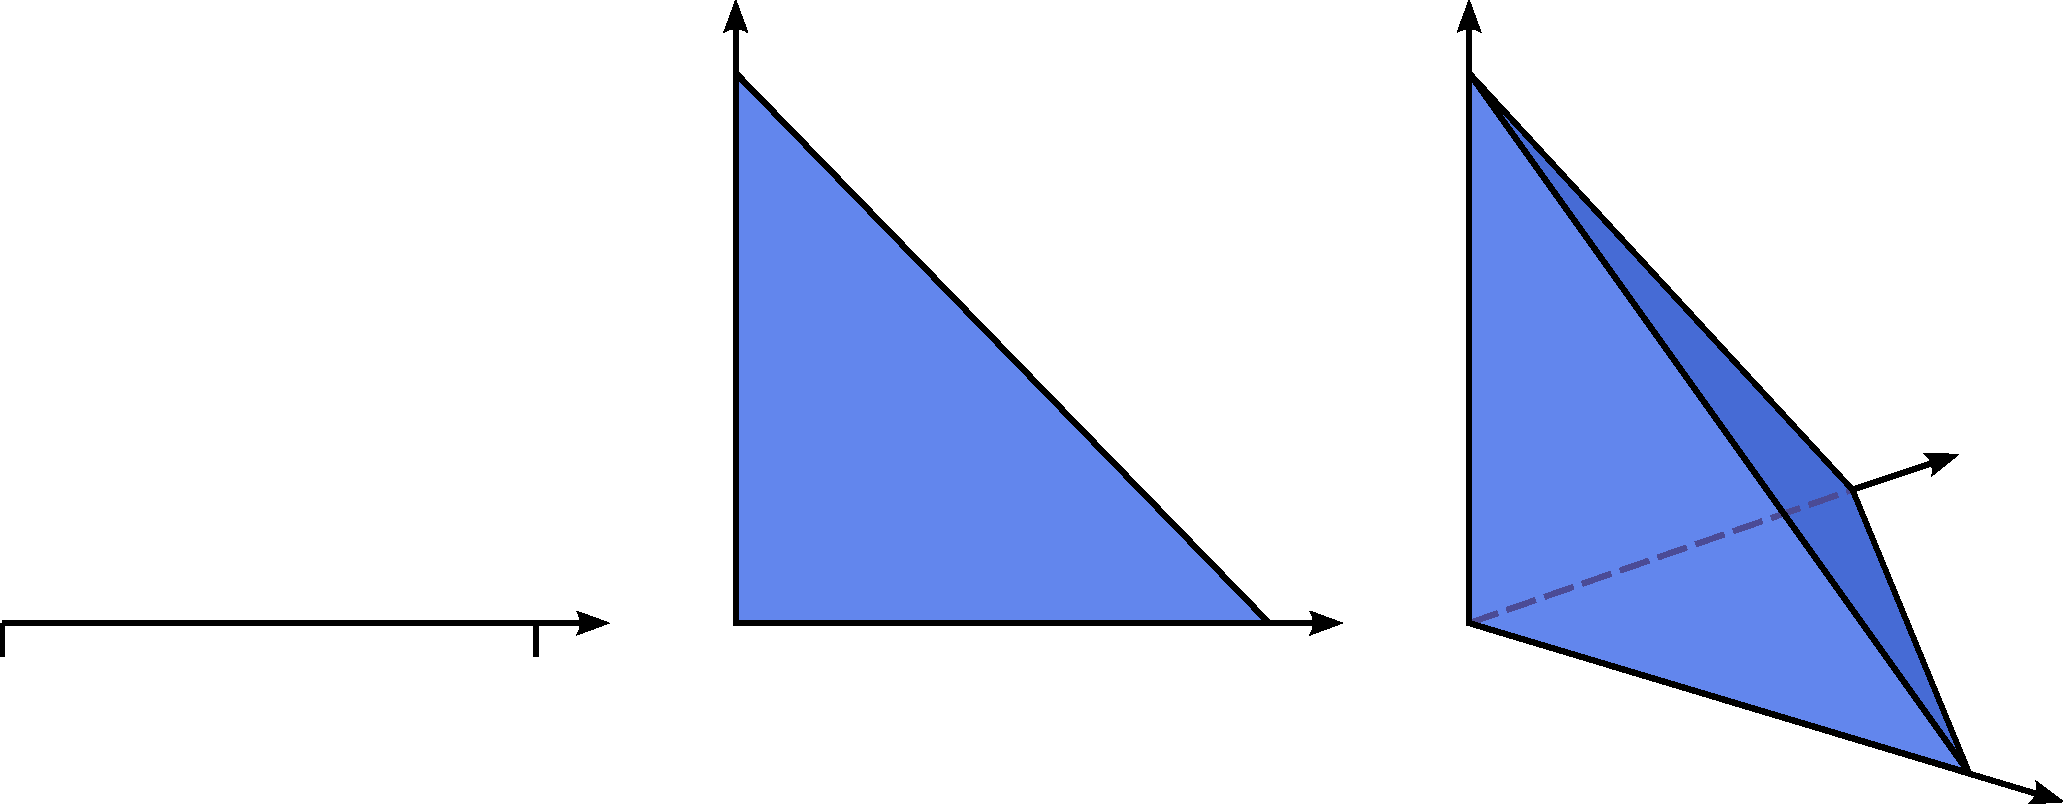
\includegraphics[width=\largefig]{chapters/kirby-7/pdf/cells.pdf}}
\end{figure}

%\begin{figure}
%  \caption{A straight triangular cell (left) and curved triangular
%      cell (right).}
%  \label{fig:shapes,curved}}
%  \includegraphics[width=\largefig,height=3cm]{chapters/kirby-7/pdf/straight_and_cur%ved_triangles.pdf}
%\end{figure}

\enlargethispage{-5pt}
\vspace*{4pt}
\subsection{The finite element definition}

Once a domain~$\Omega$ has been partitioned into cells, one may define
a local function space $\CiarletSpace$ on each cell $T$ and use these
local function spaces to build the global function space~$V_h$. A cell
$T$ together with a local function space $\CiarletSpace$ and a set of
rules for describing the functions in $\CiarletSpace$ is called a
\emph{finite element}. This definition was first
formalized by~\citet{Ciarlet1976} and it remains the standard
formulation today~\citep{BrennerScott2008}. The formal definition
reads as follows: a finite element is a triple $(T,
\CiarletSpace, \mathcal{L})$, where
\femdefinition{}

As an example, consider the standard linear Lagrange finite element on
the triangle in~Figure~\ref{fig:P1}. The cell~$T$ is given by the
triangle and the space $\CiarletSpace$ is given by the space of first
degree polynomials on $T$ (a space of dimension three). As a basis for
$\CiarletSpace'$, we may take point evaluation at the three vertices
of $T$; that is,
\begin{equation}
  \begin{split}
    \ell_i : \CiarletSpace \rightarrow \R,
    \\
    \ell_i(v) = v(x^i),
  \end{split}
\end{equation}
\looseness-1{}for $i=1,2,3$ where $x^i$ is the coordinate of the $i$th vertex. To
check that this is indeed a finite element, we need to verify that
$\mathcal{L}$ is a basis for $\CiarletSpace'$. This is equivalent to
the unisolvence of $\mathcal{L}$; that is, if $v\in\CiarletSpace$ and
$\ell_i(v) = 0$ for all $\ell_i$, then $v =
0$~\citep{BrennerScott2008}. For the linear Lagrange triangle, we note
that if $v$ is zero at each vertex, then $v$ must be zero everywhere,
since a plane is uniquely~determined by its values at three
non-collinear points. It follows that the linear Lagrange triangle is
indeed a finite element. In general, determining the unisolvence of
$\mathcal{L}$ may be non-trivial.

\begin{figure}
\bwfig
  \centering
  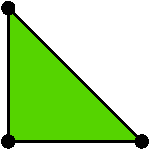
\includegraphics[width=\smallfig]{chapters/kirby-7/pdf/P1.pdf}
  \caption{The degrees of freedom of the linear Lagrange (Courant)
    triangle are given by point evaluation at the three vertices of
    the triangle.}
  \label{fig:P1}
\end{figure}

\subsection{The nodal basis}
\index{nodal basis}

Expressing finite element solutions in $V_h$ in terms of basis
functions for the local function spaces $\CiarletSpace$ may be greatly
simplified by introducing a \emph{nodal basis} for $\CiarletSpace$.  A
nodal basis $\{\phi_i\}_{i=1}^{n}$ for~$\CiarletSpace$ is a basis for
$\CiarletSpace$ that satisfies
\begin{equation} \label{eq:nodalbasis}
  \ell_i(\phi_j) = \delta_{ij}, \quad i, j = 1,2,\ldots, n.
\end{equation}
It follows that any $v \in \CiarletSpace$ may be expressed by
\begin{equation}
  v = \sum_{i=1}^{n} \ell_i(v) \phi_i.
\end{equation}
In particular, any function $v$ in $\CiarletSpace$ for the linear
Lagrange triangle is given by $v = \sum_{i=1}^3 v(x^i) \phi_i$. In
other words, the expansion coefficients of any function $v$ may be
obtained by evaluating the linear functionals in~$\mathcal{L}$
at~$v$. We shall therefore interchangeably refer to both the expansion
coefficients~$U$ of $u_h$ and the linear functionals of $\mathcal{L}$
as the \emph{degrees of freedom}.
\index{linear Lagrange element}

\begin{example}[Nodal basis for the linear Lagrange simplices]
  The nodal basis for the linear Lagrange interval with vertices at
  $x^1 = 0$ and $x^2 = 1$ is given by
  \begin{equation}
    \phi_1(x) = 1 - x, \quad
    \phi_2(x) = x.
  \end{equation}
  The nodal basis for the linear Lagrange triangle with vertices at
  $x^1 = (0, 0)$, $x^2 = (1, 0)$ and $x^3 = (0, 1)$ is given by
  \begin{equation}
    \phi_1(x) = 1 - x_1 - x_2, \quad
    \phi_2(x) = x_1, \quad
    \phi_3(x) = x_2.
  \end{equation}
  The nodal basis for the linear Lagrange tetrahedron with vertices at
  $x^1 = (0, 0, 0)$, $x^2 = (1, 0, 0)$, $x^3 = (0, 1, 0)$ and $x^4 =
  (0, 0, 1)$ is given by
  \begin{equation}
    \begin{array}{cc}
      \begin{array}{rcl}
        \phi_1(x) &=& 1 - x_1 - x_2 - x_3, \\
        \phi_3(x) &=& x_2,
      \end{array}
      &
      \begin{array}{rcl}
        \phi_2(x) &=& x_1, \\
        \phi_4(x) &=& x_3.
      \end{array}
    \end{array}
  \end{equation}
\end{example}

For any finite element $(T, \CiarletSpace, \mathcal{L})$, the nodal
basis may be computed by solving a linear system of size $n \times
n$. To see this, let $\{\psi_i\}_{i=1}^{n}$ be any basis (the
\emph{prime} basis) for $\CiarletSpace$. Such a basis is easy to
construct if $\CiarletSpace$ is a full polynomial space or may
otherwise be computed by a singular-value decomposition or a
Gram--Schmidt procedure; see~\citet{Kirby2004}. We may then make an
Ansatz for the nodal basis in terms of the prime basis:
\begin{equation}
  \phi_j = \sum_{k=1}^{n} \alpha_{jk} \psi_k, \quad j = 1,2,\ldots,n.
\end{equation}
Inserting this into~(\ref{eq:nodalbasis}), we find that
\begin{equation}
  \sum_{k=1}^{n} \alpha_{jk} \ell_i(\psi_k) = \delta_{ij}, \quad i, j = 1,2,\ldots,n.
\end{equation}
In other words, the coefficients~$\alpha$ expanding the nodal basis
functions in the prime basis may be computed by solving the linear
system
\begin{equation}
  B \alpha^{\top} = I,
\end{equation}
where $B_{ij} = \ell_i(\psi_j)$.

\subsection{The local-to-global mapping}
\index{local-to-global mapping}

Now, to define a global function space $V_h = \mathrm{span}
\{\phi_i\}_{i=1}^N$ on $\Omega$ from a given set $\{(T,
\CiarletSpace_T,\mathcal{L}_T)\}_{T\in\mesh}$ of finite elements, we
also need to specify how the local function spaces are patched
together. We do this by specifying for each cell $T \in \mesh$ a
\emph{local-to-global mapping}:
\begin{equation}
  \iota_T : [1, n_T] \rightarrow [1, N].
\end{equation}
This mapping specifies how the local degrees of freedom~$\mathcal{L}_T =
\{\ell_i^T\}_{i=1}^{n_T}$ are mapped to global degrees of
freedom~$\mathcal{L} = \{\ell_i\}_{i=1}^N$. More precisely, the global
degrees of freedom are defined by
\begin{equation} \label{eq:nodemapping}
  \ell_{\iota_T(i)}(v) = \ell^T_i(v|_T), \quad i = 1,2,\ldots,n_T,
\end{equation}
for any $v\in V_h$. Thus, each local degree of freedom~$\ell^T_i \in
\mathcal{L}_T$ corresponds to a global degree of
freedom~$\ell_{\iota_T(i)} \in \mathcal{L}$ determined by the
local-to-global mapping $\iota_T$. As we shall see, the
local-to-global mapping together with the choice of degrees of freedom
determine the continuity of the global function space~$V_h$.

For standard continuous piecewise linears, one may define the
local-to-global mapping by simply mapping each local vertex number $i$
for $i=1,2,3$ to the corresponding global vertex number
$\iota_T(i)$. For continuous piecewise quadratics, one can base the
local-to-global mapping on global vertex and edge numbers as
illustrated in Figure~\ref{fig:dofmap} for a simple mesh consisting of
two triangles.

\begin{figure}
\bwfig
  \centering
  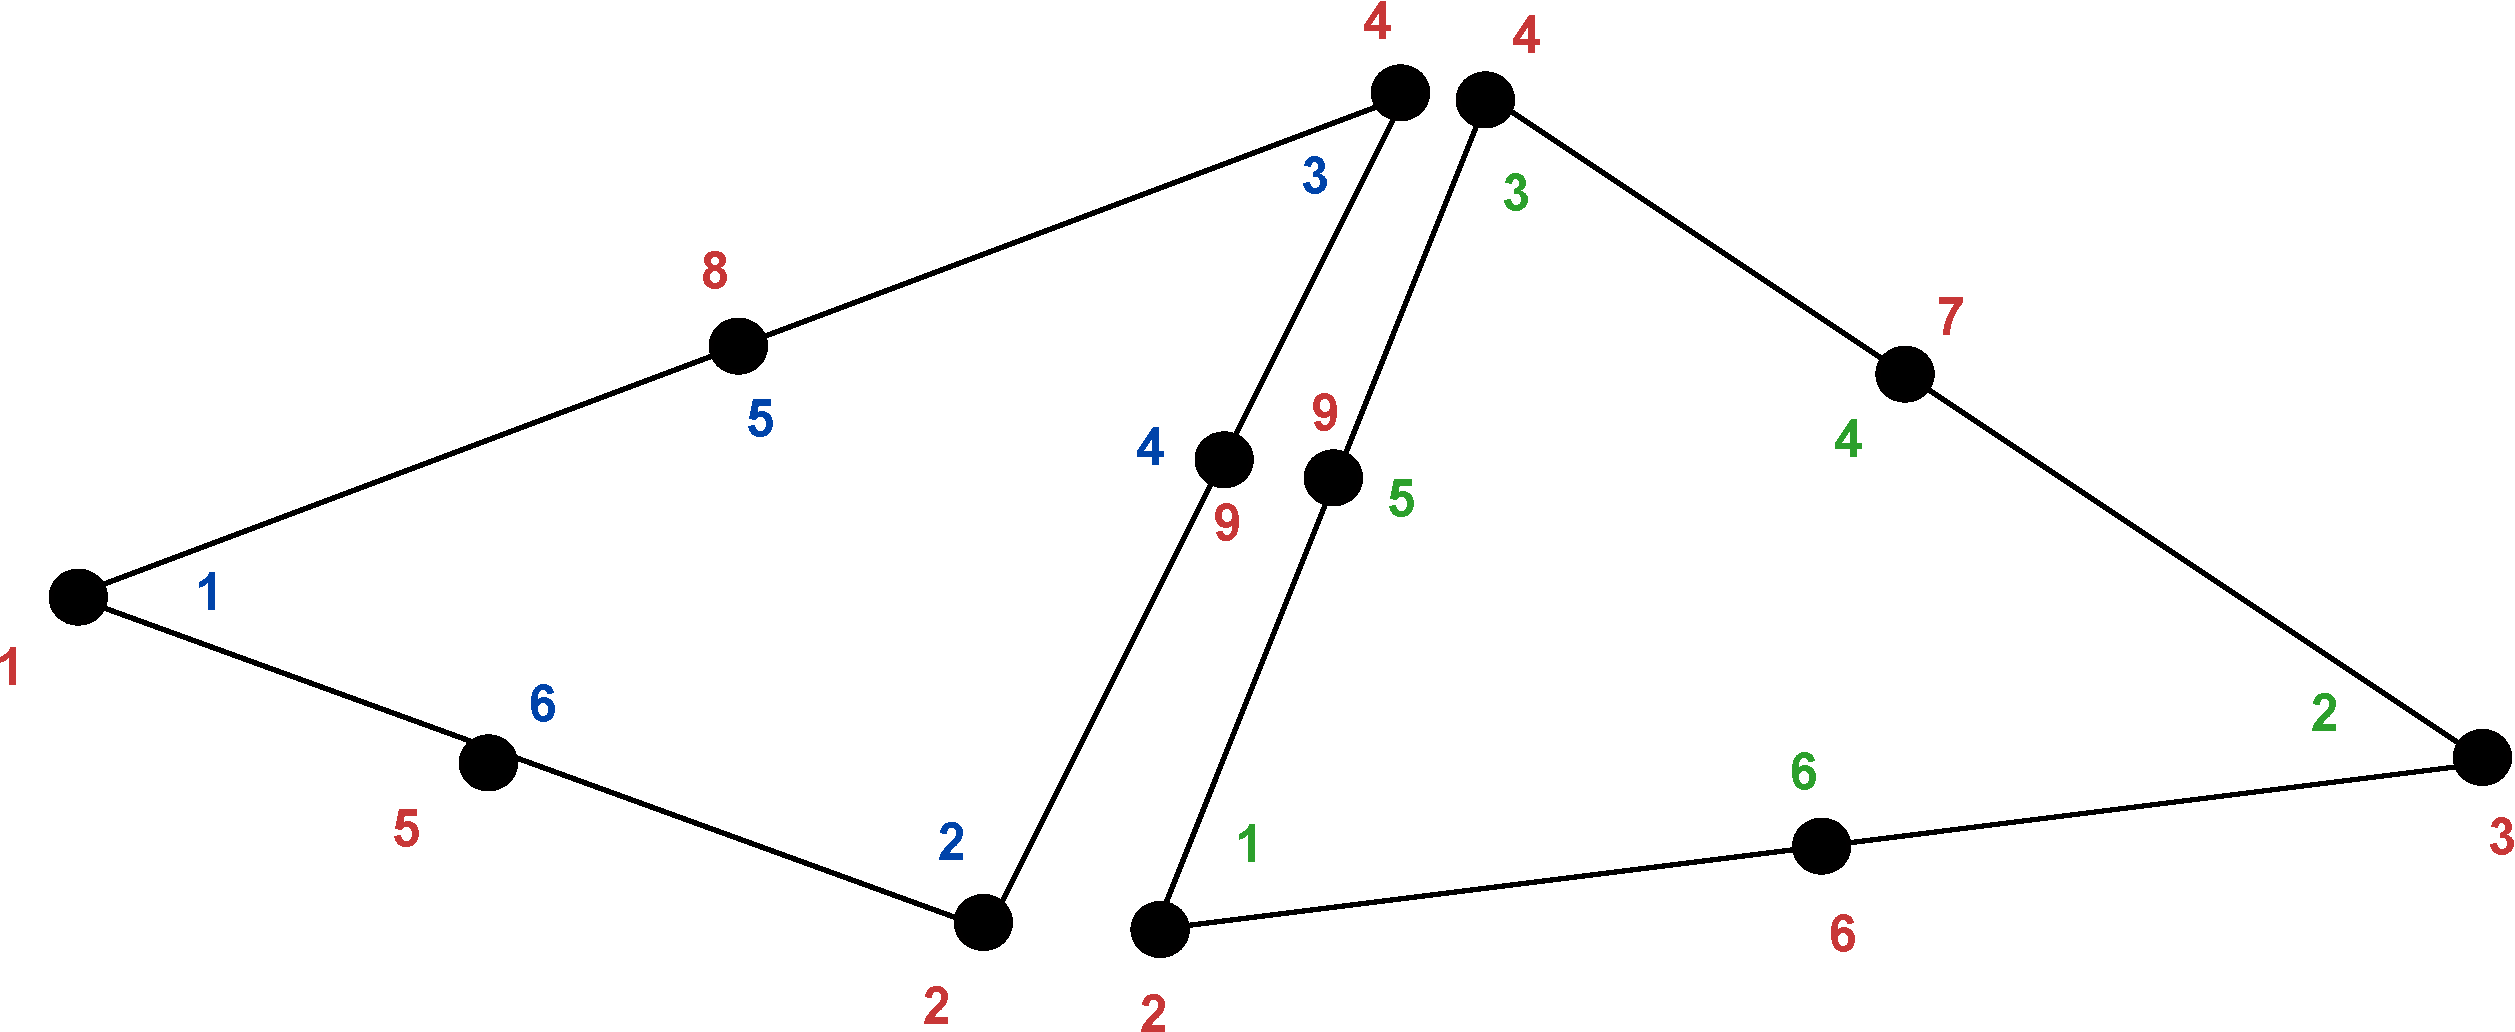
\includegraphics[width=\largefig]{chapters/kirby-7/pdf/dofmap.pdf}
  \caption{Local-to-global mapping for a simple mesh consisting of
    two triangles. The six local degrees of freedom of the left
    triangle ($T$) are mapped to the global degrees of freedom
    $\iota_T(i) = 1, 2, 4, 9, 8, 5$ for $i = 1, 2, \ldots, 6$, and
    the six local degrees of freedom of the right triangle ($T'$)
    are mapped to $\iota_{T'}(i) = 2, 3, 4, 7, 9, 6$ for $i = 1, 2,
    \ldots, 6$.}
  \label{fig:dofmap}
\end{figure}

\subsection{The global function space}
One may now define the global function space $V_h$ as the set of
functions on $\Omega$ satisfying the following pair of conditions. We
first require that
\begin{equation}
  v |_T \in \CiarletSpace_T \quad \foralls T \in \mesh;
\end{equation}
that is, the restriction of $v$ to each cell~$T$ lies in the local
function space~$\CiarletSpace_T$. Second, we require that for any pair
of cells $(T, T') \in \mesh \times \mesh$ and any pair~$(i, i') \in
[1,n_T] \times [1,n_{T'}]$ satisfying
\begin{equation}
  \iota_T(i) = \iota_{T'}(i'),
\end{equation}
it holds that
\begin{equation} \label{eq:constraint}
  \ell^T_i(v|_T) = \ell^{T'}_{i'}(v|_{T'}).
\end{equation}
In other words, if two local degrees of freedom $\ell_i^T$ and
$\ell^{T'}_{i'}$ are mapped to the same global degree of freedom, then
they must agree for each function $v \in V_h$. Here, $v|_T$ denotes
(the continuous extension of the) restriction of $v$ to the interior
of $T$. This is illustrated in Figure~\ref{fig:femspace} for the space
of continuous piecewise quadratics obtained by patching together two
quadratic Lagrange triangles.

\begin{figure}
  \centering
  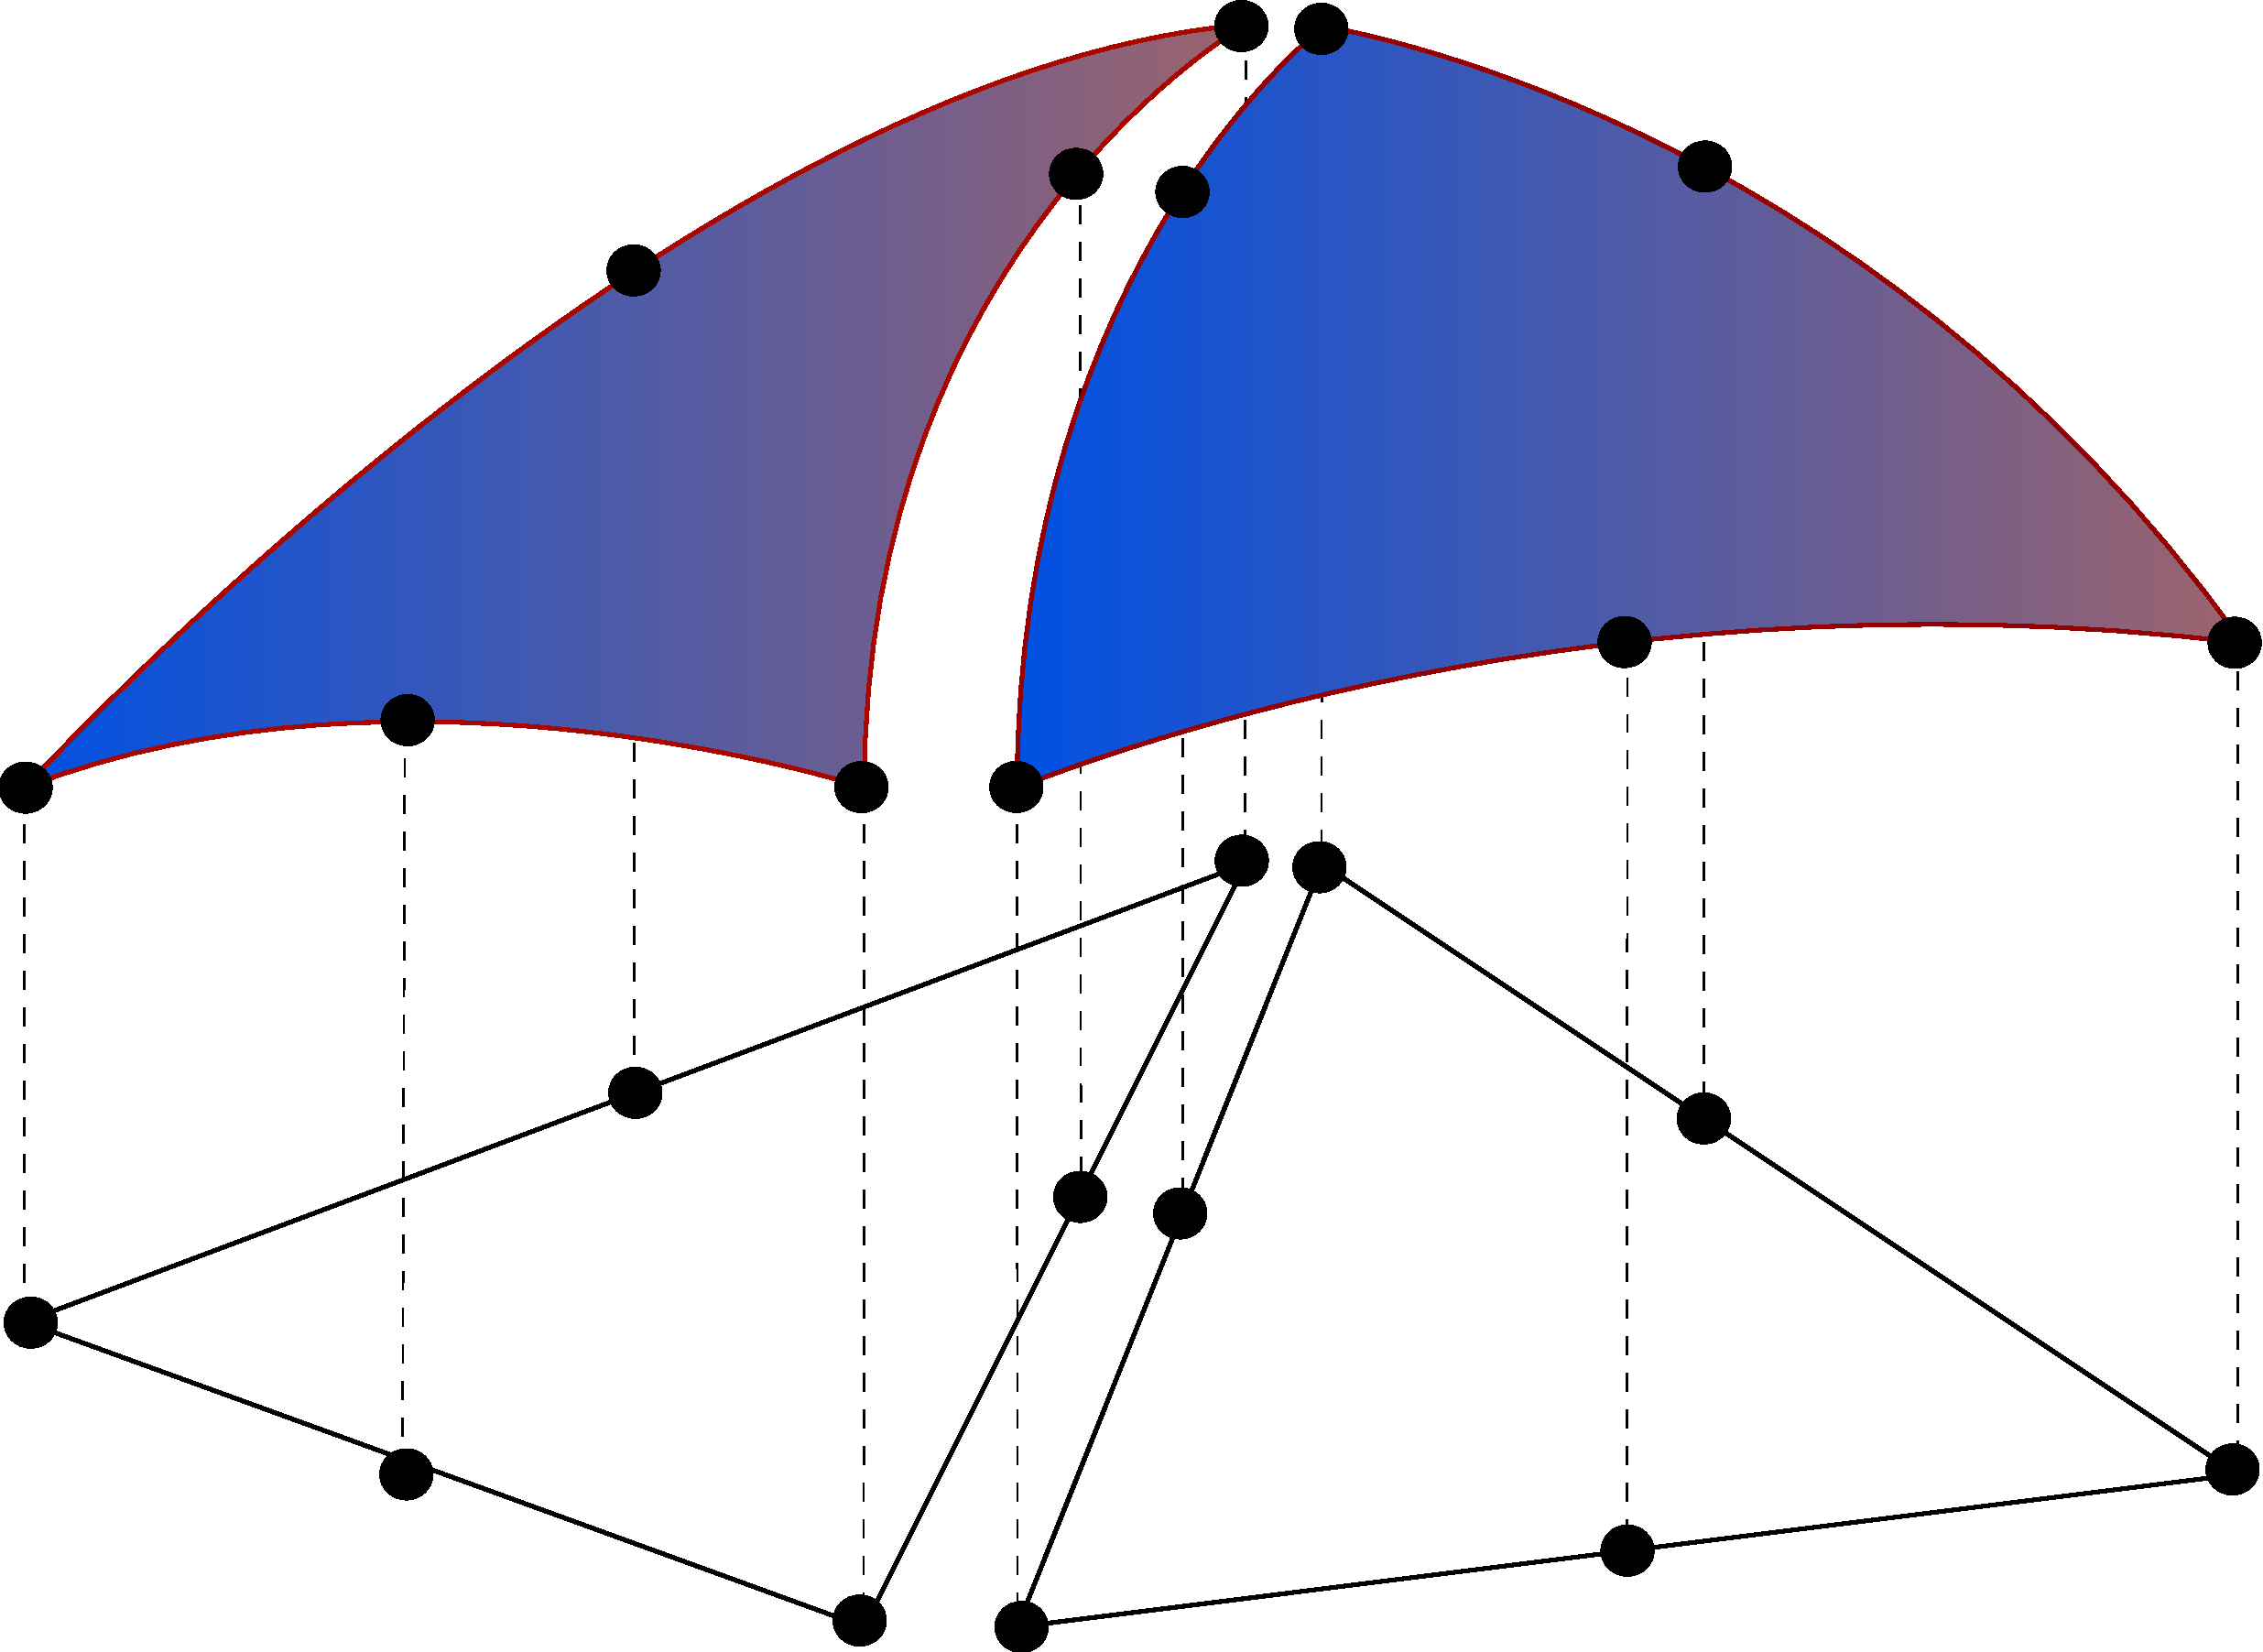
\includegraphics[width=\largefig]{chapters/kirby-7/pdf/femspace.pdf}
  \caption{Patching together a pair of quadratic local function
    spaces on a pair of cells $(T, T')$ to form a global continuous
    piecewise quadratic function space on $\Omega = T \cup T'$.}
  \label{fig:femspace}
\end{figure}

Note that by this construction, the functions in $V_h$ are undefined
on cell boundaries, unless the constraints (\ref{eq:constraint}) force
the functions in $V_h$ to be continuous on cell boundaries. However,
this is usually not a problem, since we can perform all operations on
the restrictions of functions to the local cells.

The local-to-global mapping together with the choice of degrees of
freedom determine the continuity of the global function space~$V_h$.
For the linear Lagrange triangle, choosing the degrees of freedom as
point evaluation at the vertices ensures that all functions in $V_h$
must be continuous at the two vertices of the common edge of any pair
of adjacent triangles, and therefore along the entire common edge. It
follows that the functions in $V_h$ are continuous throughout the
domain~$\Omega$. As a consequence, the space of piecewise linears
generated by the Lagrange triangle is $H^1$-conforming; that is, $V_h
\subset H^1(\Omega)$.

\index{Crouzeix--Raviart element}
\index{Brezzi--Douglas--Marini element}
\index{\nedelec{} element}
%
One may also consider degrees of freedom defined by point evaluation
at the midpoint of each edge. This is the so-called Crouzeix--Raviart
triangle. The corresponding global Crouzeix--Raviart space $V_h$ is
consequently continuous only at edge midpoints. The Crouzeix--Raviart
triangle is an example of an $H^1$-\emph{nonconforming} element; that
is, the function space $V_h$ constructed from a set of
Crouzeix--Raviart elements is not a subspace of $H^1$. Other choices
of degrees of freedom may ensure continuity of normal components, like
for the $\Hdiv$-conforming Brezzi--Douglas--Marini elements, or
tangential components, as for the $\Hcurl$-conforming \nedelec{}
elements. In Chapter~\ref{chap:kirby-6}, other examples of elements
are given which ensure different kinds of continuity by the choice of
degrees of freedom and local-to-global mapping.

\enlargethispage{12pt}

\vspace*{-6pt}\subsection{The mapping from the reference element}
\index{mapping from reference element}
\index{affine mapping}

As we have seen, the global function space $V_h$ may be described by a
mesh $\mesh$, a set of finite elements
$\{(T,\CiarletSpace_T,\mathcal{L}_T)\}_{T\in\mesh}$ and a set of
local-to-global mappings $\{\iota_T\}_{T\in\mesh}$. We may simplify
this description further by introducing a \emph{reference finite
  element} $(\hat{T},\hat{\CiarletSpace},\hat{\mathcal{L}})$,
where $\hat{\mathcal{L}} =
\{\hat{\ell}_1,\hat{\ell}_2,\ldots,\hat{\ell}_{\hat{n}}\}$, and
a set of invertible mappings $\{F_T\}_{T\in\mesh}$ that map the
reference cell~$\hat{T}$ to the cells of the mesh:
\begin{equation}
  T = F_T(\hat{T}) \quad \foralls T \in \mesh.
\end{equation}
This is illustrated in Figure~\ref{fig:kirby-7:affinemap}. Note that
$\hat{T}$ is generally not part of the mesh.

\begin{figure}%10
\bwfig
%  \centering
%  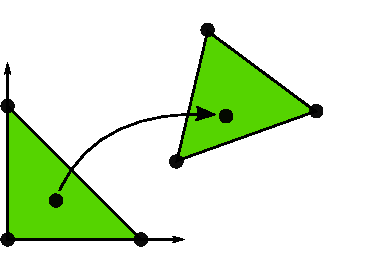
\includegraphics[width=\largefig]{chapters/kirby-7/pdf/affine_map.pdf}
  \fenicsfig{kirby-7}{affine_map}{\largefig}
  \caption{The (affine) map $F_T$ from a reference cell $\hat{T}$
    to a cell $T \in \mesh$.}
  \label{fig:kirby-7:affinemap}
\end{figure}

\index{Piola mapping}
\index{covariant Piola mapping}
\index{contravariant Piola mapping}
%
For function spaces discretizing $H^1$ as
in~(\ref{eq:poisson,varproblem}), the mapping $F_T$ is typically
\emph{affine}; that is, $F_T$ can be written in the form $F_T(\hat{x})
= A_T \hat{x} + b_T$ for some matrix $A_T \in \R^{d\times d}$ and some
vector $b_T \in \R^d$, or else \emph{isoparametric}, in which case the
components of $F_T$ are functions in $\hat{\CiarletSpace}$. For function
spaces discretizing $\Hdiv$ like
in~(\ref{eq:poisson,varproblem,mixed}) or $\Hcurl$, the appropriate
mappings are the contravariant and covariant Piola mappings which
preserve normal and tangential components, respectively;
see~\citet{RognesKirbyLogg2009}. For simplicity, we restrict the
following discussion to the case when $F_T$ is affine or
isoparametric.

For each cell $T \in \mesh$, the mapping $F_T$ generates a
function space on $T$ given by
\begin{equation}
  \CiarletSpace_T = \{ v : v = \hat{v} \circ F_T^{-1}, \quad \hat{v} \in
  \hat{\CiarletSpace} \};
\end{equation}

\pagebreak

\noindent
that is, each function $v = v(x)$ may be expressed as $v(x) =
\hat{v}(F_T^{-1}(x)) = \hat{v} \circ F_T^{-1} (x)$ for some $\hat{v}
\in \hat{\CiarletSpace}$.

The mapping $F_T$ also generates a set of degrees of freedom
$\mathcal{L}_T$ on $\CiarletSpace_T$ given by
\begin{equation}
  \mathcal{L}_T = \{ \ell_i : \ell_i(v) = \hat{\ell}_i(v \circ
  F_T), \quad i=1,2,\ldots,\hat{n} \}.
\end{equation}
The mappings $\{F_T\}_{T\in\mesh}$ thus generate from the reference
finite element~$(\hat{T},\hat{\CiarletSpace},\hat{\mathcal{L}})$ a set
of finite elements $\{(T,\CiarletSpace_T,\mathcal{L}_T)\}_{T\in\mesh}$
given by
\begin{equation} \label{eq:elementgeneration}
  \begin{split}
  T &= F_T(\hat{T}),
  \\[1ex]
  \CiarletSpace_T &= \{ v : v = \hat{v} \circ F_T^{-1}, \quad \hat{v} \in \hat{\CiarletSpace} \},
  \\[1ex]
  \mathcal{L}_T &= \{ \ell_i : \ell_i(v) = \hat{\ell}_i(v \circ F_T),
  \quad i=1,2,\ldots,\hat{n} = n_T \}.
  \end{split}
\end{equation}
By this construction, we also obtain the nodal basis functions
$\{\phi^T_i\}_{i=1}^{n_T}$ on $T$ from a set of nodal basis functions
$\{\hat{\phi}_i\}_{i=1}^{\hat{n}}$ on the reference element satisfying
$\hat{\ell}_i(\hat{\phi}_j) = \delta_{ij}$. To see this, we let
$\phi^T_i = \hat{\phi}_i \circ F_T^{-1}$ for $i=1,2,\ldots,n_T$ and
find that
\begin{equation}
  \ell^T_i(\phi^T_j)
  = \hat{\ell}_i(\phi^T_j \circ F_T)
  = \hat{\ell}_i(\hat{\phi}_j \circ F_T^{-1} \circ F_T)
  = \hat{\ell}_i(\hat{\phi}_j)
  = \delta_{ij},
\end{equation}
so $\{\phi^T_i\}_{i=1}^{n_T}$ is a nodal basis for $\CiarletSpace_T$.

We may therefore define the function space $V_h$ by specifying a
mesh~$\mesh$, a reference finite element $(\hat{T},
\hat{\CiarletSpace}, \hat{\mathcal{L}})$, a set of local-to-global
mappings $\{\iota_T\}_{T\in\mesh}$ and a set of mappings
$\{F_T\}_{T\in\mesh}$ from the reference cell $\hat{T}$. Note that in
general, the mappings need not be of the same type for all cells $T$
and not all finite elements need to be generated from the same
reference finite element. In particular, one could employ a different
(higher-degree) isoparametric mapping for cells on a curved boundary.

\index{affine equivalence}
\index{Hermite element}
%
The above construction is valid for so-called affine-equivalent
elements~\citep{BrennerScott2008} like the family of $H^1$-conforming
Lagrange finite elements. A similar construction is possible for
$\Hdiv$- and $\Hcurl$-conforming elements, like the
Brezzi--Douglas--Marini and \nedelec{} elements, where an appropriate
Piola mapping must be used to map the basis functions (while an affine
map may still be used to map the geometry). However, not all finite
elements may be generated from a reference finite element using this
simple construction. For example, this construction fails for the
family of Hermite finite
elements~\citep{Ciarlet2002,BrennerScott2008}.

\enlargethispage{12pt}

%------------------------------------------------------------------------------
\section{Finite element solvers}
\index{linear solvers}

Finite elements provide a powerful methodology for discretizing
differential equations, but solving the resulting algebraic systems
also presents a challenge, even for linear systems. Good solvers must
handle the sparsity and possible ill-conditioning of the algebraic
system, and also scale well on parallel computers.  The linear solve
is a fundamental operation not only in linear problems, but also
within each iteration of a nonlinear solve via Newton's method, an
eigenvalue solve, or time-stepping.

A classical approach that has been revived recently is direct
solution, based on Gaussian elimination.  Thanks to techniques
enabling parallel scalability and recognizing block structure,
packages such as UMFPACK~\citep{Davis2004} and SuperLU~\citep{Li2005}
have made direct methods competitive for quite large problems.

The 1970s and 1980s saw the advent of modern iterative methods. These
grew out of classical iterative methods such as relaxation methods and
the conjugate gradient iteration of~\citet{HestenesStiefel1952}. These
techniques can use much less memory than direct methods and are easier
to parallelize.

\pagebreak

Multigrid methods~\citep{Brandt1977,Wesseling1992} use relaxation
techniques on a hierarchy of meshes to solve elliptic equations,
typically for symmetric problems, in nearly linear time. However, they
require a hierarchy of meshes that may not always be available.  This
motivated the introduction of \emph{algebraic} multigrid methods (AMG)
that mimic mesh coarsening, working only on the matrix entries.
Successful AMG distributions include the Hypre
package~\citep{FalgoutYang2002} and the ML package distributed as part
of Trilinos~\citep{HerouxBartlettHowleEtAl2005}.

\index{preconditioner}
%
Krylov methods such as conjugate gradients and
GMRES~\citep{SaadSchultz1986} generate a sequence of approximations
converging to the solution of the linear system. These methods are
based only on the matrix--vector product.  The performance of these
methods is significantly improved by use of \emph{preconditioners},
which transform the linear system
\begin{equation}
AU = b
\end{equation}
into
\begin{equation}
P^{-1} A U = P^{-1} b,
\end{equation}
which is known as left preconditioning. The preconditioner $P^{-1}$
may also be applied from the right by recognizing that $A U = (A
P^{-1}) (P U)$ and solving the modified system for the matrix $A
P^{-1}$, followed by an additional solve to obtain $U$ from the
solution $PU$. To ensure good convergence, the preconditioner $P^{-1}$
should be a good approximation of $A^{-1}$. Some preconditioners are
strictly algebraic, meaning they only use information available from
the entries of \( A \). Classical relaxation methods such as
Gauss--Seidel may be used as preconditioners, as can so-called
incomplete
factorizations~\citep{Manteuffel1980,Axelsson1986,Saad1994}. Multigrid,
whether geometric or algebraic, also can serve as a powerful
preconditioner. Other kinds of preconditioners require special
knowledge about the differential equation being solved and may require
new matrices modeling related physical processes.  Such methods are
sometimes called \emph{physics-based} preconditioners. An automated
system, such as FEniCS, provides an interesting opportunity to assist
with the development and implementation of these powerful but less
widely used methods.

Fortunately, many of the methods discussed here are included in modern
libraries such as PETSc \citep{BalayBuschelmanEijkhoutEtAl2004} and
Trilinos~\citep{HerouxBartlettHowleEtAl2005}. FEniCS typically
interacts with the solvers discussed here through these packages and
so mainly need to be aware of the various methods at a high level,
such as when the various methods are appropriate and how to access
them.

%------------------------------------------------------------------------------
\section{Finite element error estimation and adaptivity}
\index{error estimation}
\index{residual}

The error~$e = u - u_h$ in a computed finite element solution~$u_h$
approximating the exact solution~$u$ of~(\ref{eq:varproblem}) may be
estimated either \emph{a~priori} or \emph{a~posteriori}.

\emph{A~priori} error estimates express the error in terms of the
regularity of the exact (unknown) solution and may give useful
information about the order of convergence of a finite element
method. \emph{A~posteriori} error estimates express the error in terms
of computable quantities like the residual and (possibly) the solution
of an auxiliary dual problem, as described below.

\subsection{\emph{A priori} error analysis}
\index{\emph{a priori} error estimate}

We consider the linear variational problem~(\ref{eq:varproblem}). We
first assume that the bilinear form~$a$ and the linear form~$L$ are
continuous (bounded); that is, there exists a constant $C > 0$ such
that
\begin{equation} \label{eq:continuity}
  \begin{split}
    a(v, w) &\leqslant C \|v\|_V \|w\|_V,
    \\
    L(v) &\leqslant C \|v\|_V,
  \end{split}
\end{equation}
for all $v, w \in V$. For simplicity, we assume in this section that
$V = \hat{V}$ is a Hilbert space. For (\ref{eq:poisson}), this
corresponds to the case of homogeneous Dirichlet boundary conditions
and $V = H^1_0(\Omega)$. Extensions to the general case $V \neq
\hat{V}$ are possible; see for example~\citet{OdenDemkowicz1996}. We
further assume that the bilinear form $a$ is coercive ($V$-elliptic);
that is, there exists a constant $\alpha > 0$ such that
\begin{equation} \label{eq:coercivity}
  a(v, v) \geqslant \alpha \|v\|_V^2,
\end{equation}
for all $v \in V$. It then follows by the Lax--Milgram
theorem~\citep{LaxMilgram1954} that there exists a unique solution~$u
\in V$ to the variational problem~(\ref{eq:varproblem}).

To derive an \emph{a~priori} error estimate for the approximate
solution $u_h$ defined by the discrete variational
problem~(\ref{eq:varproblem,discrete}), we first note that
\begin{equation}
  a(u - u_h, v) = a(u, v) - a(u_h, v) = L(v) - L(v) = 0
\end{equation}
for all $v \in V_h \subset V$ (the Galerkin orthogonality). By the
coercivity and continuity of the bilinear form~$a$, we find that
\begin{equation}
  \begin{split}
    \alpha \|u - u_h\|_V^2
    &\leqslant a(u - u_h, u - u_h)
    = a(u - u_h, u - v) + a(u_h - u, v - u_h)
    \\
    &= a(u - u_h, u - v) \leqslant C \|u - u_h\|_V \, \|u - v\|_V.
  \end{split}
\end{equation}
for all $v \in V_h$. It follows that
\begin{equation} \label{eq:ceaslemma}
  \|u - u_h\|_V
  \leqslant \frac{C}{\alpha} \|u - v\|_V \quad \foralls v \in V_h.
\end{equation}
\index{Cea's lemma}
%
The estimate (\ref{eq:ceaslemma}) is referred to as Cea's lemma. We
note that when the bilinear form~$a$ is symmetric, it is also an inner
product. We may then take $\|v\|_V = \sqrt{a(v, v)}$ and $C = \alpha =
1$. In this case, $u_h$ is the $a$-projection onto $V_h$ and Cea's
lemma states that
\begin{equation}
  \|u - u_h\|_V \leqslant \|u - v\|_V \quad \foralls v \in V_h;
\end{equation}
that is, $u_h$ is the best possible solution of the variational
problem~(\ref{eq:varproblem}) in the subspace $V_h$. This is
illustrated in Figure~\ref{fig:ceaslemma}.

\begin{figure}
\bwfig
  \centering
  \fenicsfig{kirby-7}{projection}{\largefig}
  \caption{If the bilinear form~$a$ is symmetric, then the finite
    element solution~$u_h \in V_h \subset V$ is the $a$-projection
    of $u \in V$ onto the subspace $V_h$ and is consequently the
    best possible approximation of $u$ in the subspace $V_h$ (in the
    norm defined by the bilinear form~$a$). This follows by the Galerkin orthogonality
    $\inner{u - u_h}{v}_a \equiv a(u - u_h, v) = 0$ for all $v \in V_h$.}
  \label{fig:ceaslemma}
\end{figure}

Cea's lemma together with a suitable interpolation estimate now yields
an \emph{a~priori} error estimate for $u_h$. By choosing $v = \pi_h
u$, where $\pi_h : V \rightarrow V_h$ is an interpolation operator
into $V_h$, we find that
\begin{equation} \label{eq:apriori}
  \|u - u_h\|_V
  \leqslant \frac{C}{\alpha} \|u - \pi_h u\|_V
  \leqslant \frac{C C_i}{\alpha} \|h^p D^{q + 1} u\|_{L^2},
\end{equation}
where $C_i$ is an interpolation constant and the values of $p$ and $q$
depend on the accuracy of interpolation and the definition of
$\|\cdot\|_V$. For the solution of Poisson's equation in $V = H^1_0$,
we have $C = \alpha = 1$ and $p = q = 1$.

\subsection{\emph{A posteriori} error analysis}
\index{\emph{a priori} error estimate}

\paragraph{Energy norm error estimates.}

The continuity and coercivity of the bilinear form~$a$ also allow the
derivation of an \emph{a~posteriori} error estimate. This type of error
estimate is obtained by relating the size of the error to the size of
the (weak) residual $r : \hat{V} \rightarrow \R$ defined by
\begin{equation} \label{eq:residual,weak}
  r(v) = L(v) - a(u_h, v).
\end{equation}
Note that the weak residual is formally related to the \emph{strong
  residual} $R \in \hat{V}'$ by $r(v) = \inner{R}{v}$ for all $v \in
\hat{V}$.

We first note that the $V$-norm of the error $e = u - u_h$ is
equivalent to the $V'$-norm of the residual $r$. To see this, note
that by the continuity of the bilinear form~$a$, we have
\begin{equation}
  r(v)
  = L(v) - a(u_h, v) = a(u, v) - a(u_h, v) = a(u - u_h, v)
  \leqslant C \|u - u_h\|_V \, \|v\|_V.
\end{equation}
Furthermore, by coercivity, we find that
\begin{equation}
  \alpha \|u - u_h\|^2_V
  \leqslant a(u - u_h, u - u_h)
  = a(u, u - u_h) - a(u_h, u - u_h)
  = L(u - u_h) - a(u_h, u - u_h) = r(u - u_h).
\end{equation}
It follows that
\begin{equation} \label{eq:aposteriori}
  \alpha \|u - u_h\|_V \leqslant \|r\|_{V'} \leqslant C \|u - u_h\|_V,
\end{equation}
where $\|r\|_{V'} = \sup_{v \in V, v \neq 0} r(v)/ \|v\|_V$.

The estimates (\ref{eq:apriori}) and (\ref{eq:aposteriori}) are
sometimes referred to as \emph{energy norm} error estimates. This is
the case when the bilinear form~$a$ is symmetric and thus defines an
inner product. One may then take $\|v\|_V = \sqrt{a(v, v)}$ and $C =
\alpha = 1$. In this case, it follows that
\begin{equation} \label{eq:aposteriori,energynorm}
  \eta \equiv \|e\|_V = \|r\|_{V'}.
\end{equation}
The term energy norm refers to $a(v, v)$ corresponding to physical
energy in many applications.


\vspace*{-6pt}\paragraph{Goal-oriented error estimates.}
\index{goal-oriented error estimate}
\index{dual problem}

The classical \emph{a~priori} and \emph{a~posteriori} error estimates
(\ref{eq:apriori}) and (\ref{eq:aposteriori}) relate the $V$-norm of
the error $e = u - u_h$ to the regularity of the exact solution~$u$
and the residual $r = L(v) - a(u_h, v)$ of the finite element
solution~$u_h$, respectively. However, in applications it is often
necessary to control the error in a certain \emph{output functional}
$\mathcal{M} : V \rightarrow \R$ of the computed solution to within
some given tolerance $\epsilon > 0$. Typical functionals are average
values of the computed solution, such as the lift or drag of an object
immersed in a flow field. In these situations, one would ideally like
to choose the finite element space $V_h \subset V$ such that the
finite element solution~$u_h$ satisfies
\begin{equation}
  \eta \equiv |\mathcal{M}(u) - \mathcal{M}(u_h)| \leqslant \epsilon
\end{equation}
with minimal computational work. We assume here that both the output
functional and the variational problem are linear, but the analysis
may be easily extended to the\vadjust{\pagebreak} full nonlinear
case~[\citeauthor{ErikssonEstepEtAl1995}\citeyear{ErikssonEstepEtAl1995},\,\citeauthor{BeckerRannacher2001}
\citeyear{BeckerRannacher2001}].

To estimate the error in the output functional~$\mathcal{M}$, we
introduce an auxiliary \emph{dual} problem: find $z \in V^*$ such that
\begin{equation} \label{eq:varproblem,dual}
  a^*(z, v) = \mathcal{M}(v) \quad \foralls v \in \hat{V}^*.
\end{equation}
We note here that the functional~$\mathcal{M}$ enters as data in the
dual problem. The dual (adjoint) bilinear form $a^* : V^* \times
\hat{V}^* \rightarrow \R$ is defined by
\begin{equation}
  a^*(v, w) = a(w, v) \quad \foralls (v, w) \in V^* \times \hat{V}^*.
\end{equation}
The dual trial and test spaces are given by
\begin{equation}
  \begin{split}
    V^* &= \hat{V},
    \\
    \hat{V}^* &= V_0 = \{v - w : v, w \in V\};
  \end{split}
\end{equation}
that is, the dual trial space is the primal test space and the dual
test space is the primal trial space modulo boundary conditions. In
particular, if $V = u_0 + \hat{V}$ then
$V^* = \hat{V}^* = \hat{V}$, and both the dual test and trial
functions vanish at Dirichlet boundaries. The definition of the dual
problem leads us to the following representation of the error:
\begin{equation}
  \begin{split}
    \mathcal{M}(u) - \mathcal{M}(u_h)
    &= \mathcal{M}(u - u_h)
    \\
    &= a^*(z, u - u_h)
    \\
    &= a(u - u_h, z)
    \\
    &= L(z) - a(u_h, z)
    \\
    &= r(z).
  \end{split}
\end{equation}
We find that the error is exactly represented by the residual of the
dual solution:
\begin{equation} \label{eq:aposteriori,dual}
  \mathcal{M}(u) - \mathcal{M}(u_h) = r(z).
\end{equation}

\subsection{Adaptivity}
\index{adaptivity}

As seen above, one may estimate the error in a computed finite element
solution~$u_h$ in the $V$-norm or an output functional by estimating
the size of the residual~$r$.  This may be done in several different
ways. The estimate typically involves integration by parts to recover
the strong element-wise residual of the original PDE, possibly in
combination with the solution of local problems over cells or patches
of cells. In the case of the standard piecewise linear finite element
approximation of Poisson's equation~(\ref{eq:poisson}), one may obtain
the following estimate:
\begin{equation}
  \|u - u_h\|_V \equiv \|\nabla e\|_{L^2} \leqslant C
  \left(
  \sum_{T\in\mesh} h_T^2 \|R\|_{T}^2 +
  h_T \|[\partial_n u_h]\|_{\partial T}^2
  \right)^{1/2},
\end{equation}
where $R|_T = f|_T + \Delta u_h|_T$ is the strong residual, $h_T$
denotes the mesh size (the diameter of the smallest circumscribed
sphere around each cell~$T$) and $[\partial_n u_h]$ denotes the jump
of the normal derivative across mesh facets. For a derivation of this
estimate, see for example~\citet{ElmanSilvesterWathen2005}. Letting
$\eta_T^2 = h_T^2 \|R\|_{T}^2 + h_T \|[\partial_n u_h]\|_{\partial
  T}^2$, we obtain the estimate
\begin{equation}
  \|u - u_h\|_V \leqslant \eta_h \equiv C \left( \sum_T \eta_T^2 \right)^{1/2}.
\end{equation}

\index{D\"orfler marking}
%
An adaptive algorithm seeks to determine a mesh size $h = h(x)$ such
that $\eta_h \leqslant \epsilon$. Starting from an initial coarse
mesh, the mesh is successively refined in those cells where the error
indicator $\eta_T$ is large. Several strategies are available, such as
refining the top fraction of all cells where $\eta_T$ is large, say
the first $20\%$ of all cells ordered by the size of $\eta_T$. Other strategies
include refining all cells where $\eta_T$ is above a certain fraction
of $\max_{T\in\mesh} \eta_T$, or refining a top fraction of all cells
such that the sum of their error indicators account for a significant
fraction of $\eta_h$ (so-called \emph{D\"orfler
  marking}~\citep{Dorfler1996}).

\index{efficiency index}
%
Once the mesh has been refined, a new solution and new error
indicators can be computed. The process is then repeated until either
$\eta_h \leqslant \epsilon$ (the stopping criterion) or the available
resources (CPU time and memory) have been exhausted. The adaptive
algorithm yields a sequence of successively refined meshes as
illustrated in Figure~\ref{fig:refinement}. For time-dependent
problems, an adaptive algorithm needs to decide both on the local mesh
size and the size of the (local) time step as functions of space
\emph{and} time. Ideally, the error estimate $\eta_h$ is close to the
actual error, as measured by the \emph{efficiency index} $\eta_h /
\eta$ which should be close to and bounded below by one.

\begin{figure}
\bwfig
  \centering
  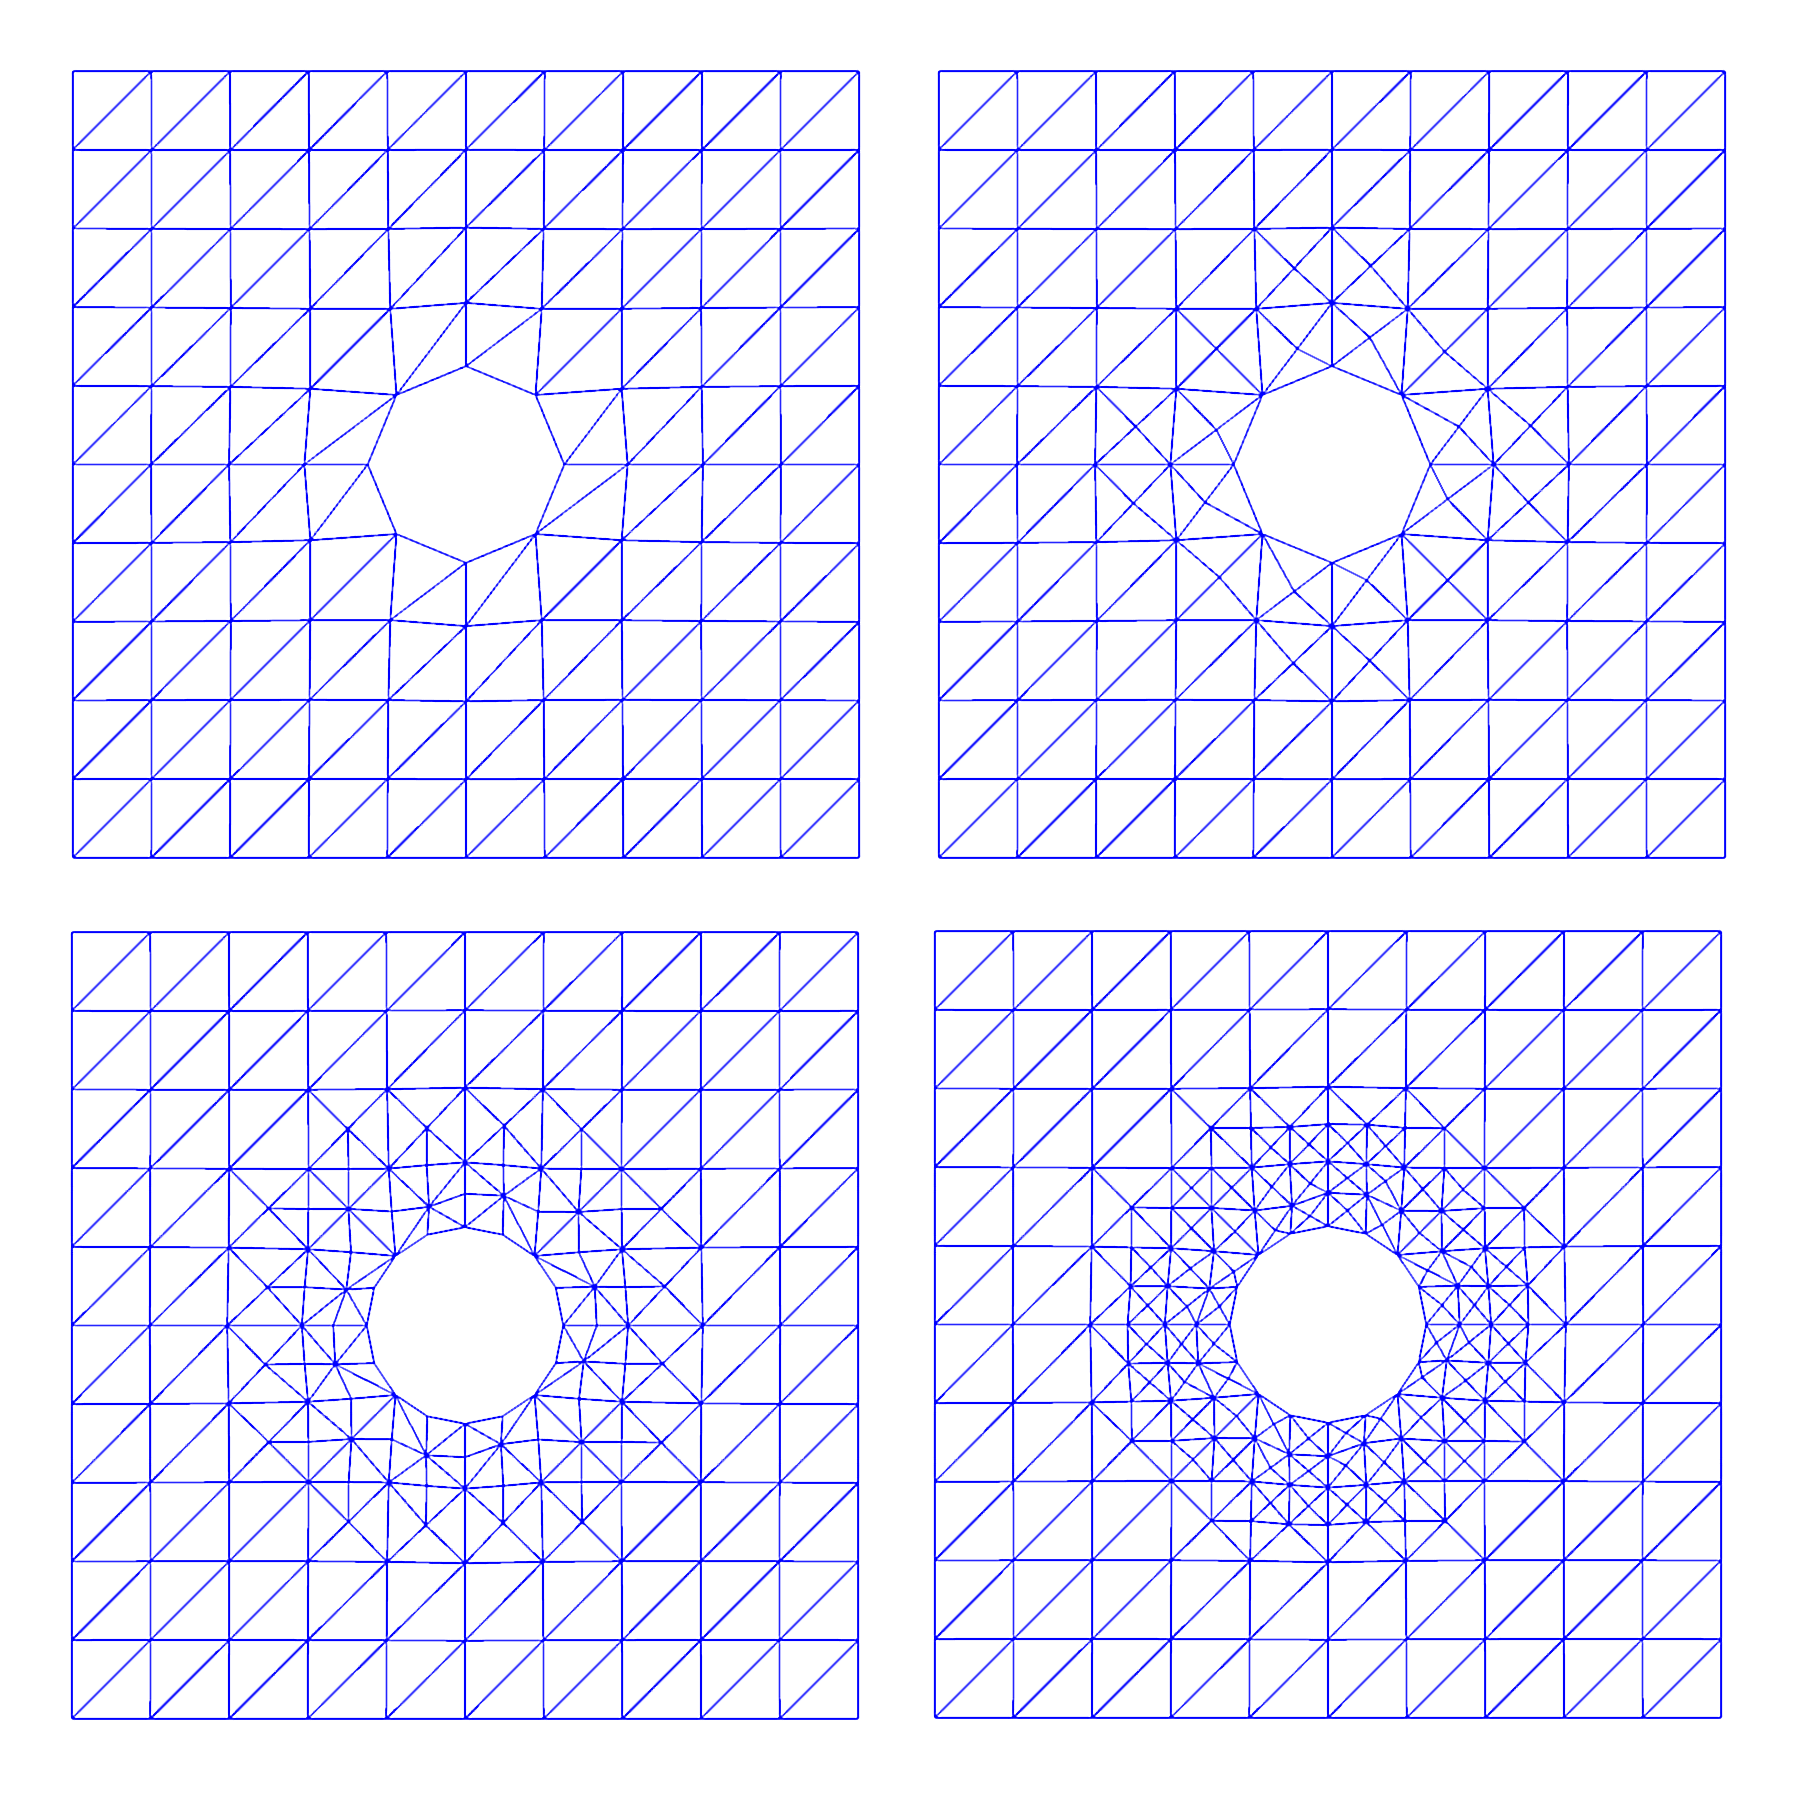
\includegraphics[width=\largefig]{chapters/kirby-7/png/refinement.png}
  \caption{A sequence of adaptively refined meshes obtained by
    successive refinement of an original coarse mesh.}
  \label{fig:refinement}
\end{figure}

%------------------------------------------------------------------------------
\section{Automating the finite element method}
\index{automation}

The FEniCS Project seeks to automate the solution of differential
equations. This is a formidable task, but it may be approached by an
automation of the finite element method. In particular, this
automation relies on the following key steps:
\begin{itemize}
\item[(i)]
  automation of discretization,
\item[(ii)]
  automation of discrete solution,
\item[(iii)]
  automation of error control.
\end{itemize}
Since its inception in~2003, the FEniCS Project has been concerned
mainly with the automation of discretization, resulting in the
development of the form compilers FFC and SyFi/SFC, the code
generation interface~UFC, the form language~UFL, and a generic
assembler implemented as part of DOLFIN. As a result, variational
problems for a large class of partial differential equations may now
be automatically discretized by the finite element method using
FEniCS. For the automation of discrete solution; that is, the solution
of linear and nonlinear systems arising from the automated
discretization of variational problems, interfaces to state-of-the-art
libraries for linear algebra have been implemented as part of
DOLFIN. Ongoing work is now seeking to automate error control by
automated error estimation and adaptivity. In the following chapters,
we return to specific aspects of the automation of the finite element
method developed as part of the FEniCS Project. The mathematical
methodology behind the FEniCS Project has also been described in
a number of scientific works. For further reading, we refer to
\citet{Logg2007a,LoggWells2010,Kirby2004,KirbyLogg2006,
AlnaesLoggMardalEtAl2009,AlnaesMardal2009b,KirbyKnepleyLoggEtAl2005,
KirbyLoggScottEtAl2006,KirbyLogg2007,KirbyLogg2008,KirbyScott2007,
Kirby2006a,OelgaardLoggWells2008,RognesKirbyLogg2009,OelgaardWells2010,
Logg2009}.

%------------------------------------------------------------------------------
\section{Historical notes}

In 1915, Boris Grigoryevich Galerkin formulated a general method for
solving differential equations~\citep{Galerkin1915}. A similar
approach was presented sometime earlier by Bubnov. Galerkin's method,
or the Bubnov--Galerkin method, was originally formulated with global
polynomials and goes back to the variational principles of Leibniz,
Euler, Lagrange, Dirichlet, Hamilton,
Castigliano \citep{Castigliano1879}, Rayleigh~\citep{Rayleigh1870} and
Ritz~\citep{Ritz1908}. Galerkin's method with piecewise polynomial
spaces $(V_h, \hat{V}_h)$ is known as the \emph{finite element
  method}. The finite element method was introduced by engineers for
structural analysis in the 1950s and was independently proposed by
Courant~\citep{Courant1943}. The exploitation of the finite element
method among engineers and mathematicians exploded in the 1960s. Since
then, the machinery of the finite element method has been expanded and
refined into a comprehensive framework for the design and analysis of
numerical methods for differential equations;
see~\citet{ZienkiewiczTaylorZhu2005firstpublishedin1967,StrangFix1973,Ciarlet1976,BeckerCareyOden1981,Hughes1987,BrennerScott2008}.
Recently, the quest for compatible (stable) discretizations of mixed
variational problems has led to the development of finite element
exterior calculus~\citep{ArnoldFalkWinther2006}.

Work on \emph{a~posteriori} error analysis of finite element methods
dates back to the pioneering work
of~\citet{BabuvskaRheinboldt1978}. Important references include the
works by~\citet{BankWeiser1985,ZienkiewiczZhu1987,
  ErikssonJohnson1991,ErikssonJohnson1995a,ErikssonJohnsonIII,ErikssonJohnson1995b,ErikssonJohnson1995c,ErikssonJohnsonLarsson1998,AinsworthOden1993}
and the reviews
papers~\citep{ErikssonEstepEtAl1995,Verfurth1994,Verfurth1999,AinsworthOden2000,BeckerRannacher2001}.
